\documentclass[]{spie}  %>>> use for US letter paper

\renewcommand{\baselinestretch}{1.0} % Change to 1.65 for double spacing
 
\usepackage{amsmath,amsfonts,amssymb}
\usepackage{graphicx}
\usepackage[colorlinks=true, allcolors=blue]{hyperref}

\title{BICEP Array cryostat and mount design}

\author[a]{Michael Crumrine}
\author[b]{}
\affil[a]{School of Physics and Astronomy, University of Minnesota,
Minneapolis, MN 55455, USA}
\affil[b]{Affiliation2, Address, City, Country}

\authorinfo{Further author information: (Send correspondence to A.A.A.)\\A.A.A.: E-mail: aaa@tbk2.edu, Telephone: 1 505 123 1234\\  B.B.A.: E-mail: bba@cmp.com, Telephone: +33 (0)1 98 76 54 32}

% Option to view page numbers
\pagestyle{empty} % change to \pagestyle{plain} for page numbers   
\setcounter{page}{301} % Set start page numbering at e.g. 301
 
\begin{document} 
\maketitle

\begin{abstract}

BICEP Array is a Cosmic Microwave Background (CMB) polarization experiment that
will begin observing at the South Pole in early 2019. This experiment replaces
the five BICEP2 style receivers that compose the Keck Array with four larger
BICEP3 style receivers observing at six frequencies from 30 to 270GHz. The
95GHz and 150GHz receivers will continue to push the already deep BICEP/Keck
CMB maps while the 30/40GHz and 220/270GHz receivers will constrain the
synchrotron and galactic dust foregrounds respectively. Here we report on the
design  and performance of the BICEP Array instruments focusing on the mount
and cryostat systems.
\end{abstract}

% Include a list of keywords after the abstract 
\keywords{Manuscript format, template, SPIE Proceedings, LaTeX}

\section{INTRODUCTION}
\label{sec:intro}  % \label{} allows reference to this section






%Begin the Introduction below the Keywords. The manuscript should not have headers, footers, or page numbers. It should be in a one-column format. References are often noted in the text and cited at the end of the paper.


\section{Cryostat Design}

BICEP array continues the successful design philosophy of
the previous Bicep / Keck receivers.An 80" tall vacuum shell contains two nested
stages with nominal operating temperatures of 50K and 4K. A cross section of
the cryostat is shown in Figure \ref{fig:cryostat}. The top section of the
vacuum jacket is sealed by an HDPE window and houses a stack of Zotefoam filters which reduce infrared loading
onto the colder stages. The intermediate 50K stage serves as a radiation
shield for the interior 4K stage. The top of this stage accommodates an
Alumina filter which further reduces infrared loading and the lower $\sim$70\%
of the intermediate 50K stage is wrapped with a 0.04" thick magnetic shield
layer composed of Amuneal A4K. The 4K stage provides radiation shielding for
the sub-K focal plane and electronics while also housing two cold Alumina
lenses and optical baffles.


The cryostat is designed to be disassembled by lifting off shells successively
from the outside in, leaving a stand-alone base behind which contains the
sub-Kelvin focal plane assembly, readout electronics, and the cooling system as shown in Figure
\ref{fig:base}. In this state, the focal plane and detector modules may be
freely accessed for maintenance and other technical activities. Access to the
underside of the focal plane and the readout electronics is provided by
hatches on the bottom side of the Vacuum shell and 50K bases. This scheme
significantly reduces the time required for disassembly when accessing the
focal plane and re-assembly afterwards by allowing critical thermal junctions
and difficult part matings to remain undisrupted.



\subsection{Thermal Architecture}


 The 50K and 4K radiation shields are cooled by the first
and second stages respectively of a Cryomech PT415-RM Pulse Tube cooler. This
cryocooler is capable of maintaining a first stage temperature of $<45$K under
a 40W load and a second stage temperature of $<4$K under a
1.5W load. The interior stages must therefore be carefully shielded in order
to stay within the thermal budget. 


The radiation absorbed by the interior stages is reduced by the use of Multi
Layer Insulation wrapped around the outside of the 50K and 4K stages. Where
there is insufficient room for uncompressed insulation, high emissivity
Aluminum tape is used to decrease the radiation absorbed by the lower
temperature surface. We calculate the total radiation loading absorbed by the
50K and 4K stages respectively to be 2.75 W and 6.9 mW respectively.


The radiation shields are additionally attached to higher temperature stages
via a low thermal conductivity support system. The front end of each shell
constrained by thin Ti-Al-4V straps which are flexible along the axial
direction of the cryostat which sees substantial thermal contraction. At the
back end, each stage is supported by six trusses each of which has two high
tensile strength / thermal conductivity rods bonded to Aluminum blocks with
Stycast epoxy. We use G10-FR4 for the backend supports between the Vacuum
shell and the 50K radiation shield but switch to Carbon Fiber between the 50K
and 4K shells due to the former's lower thermal conductivity at low
temperatures. Figure \ref{fig:supports} shows these fabricated internal
supports. We calculate the loading due to these supports to be $<2.85$W on the
50K stage and $<0.157$W on the 4K stage. 

In addition to providing radiation shielding and mount points for low
temperature optics, the 50K and 4K stages provide natural heat sinks for the
cryocables that connect the subK electronics to the exterior - room
temperature - data acquisition system.



While the pulse tube maintains the temperatures of the radiation
shields, the tiered focal plane assembly is cooled still further by a three stage Helium sorption
fridge which cools the tiers to successively lower temperatures of $2.8$K,
$340$mK and $<250$mK. Like the supports for the 4K radiation shield, the tiers
of the focal plane assembly are separated by carbon fiber support trusses
which have extremely low thermal conductivity.



\begin{figure} [ht]
	\begin{center}
		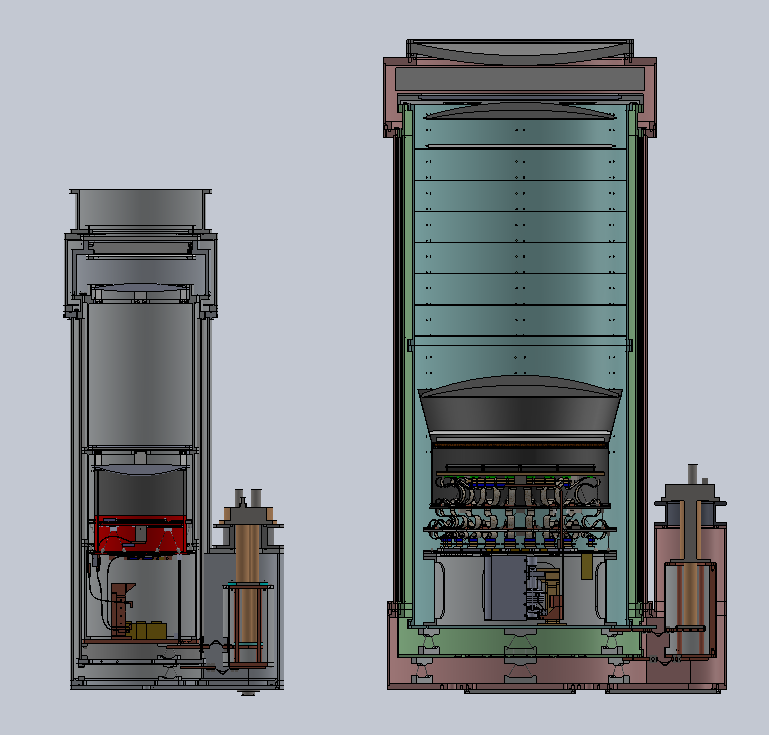
\includegraphics[scale=0.4]{BA_keck_comp.png}
	\end{center}
	\caption{A CAD cross section of a single Keck Array receiver (left) and a
	Bicep Array receiver (right). The Bicep Array cryostats more than double
	the volume of their Keck Array counterparts with mapping speed equal to
	$\sim$5 times that of a Keck receiver at the same frequency.}
	\label{fig:bavskeck}
\end{figure}


\subsection{Copper Braid Heat Straps}

The heat straps connecting the pulse tube cooler to the 50K and 4K stages of
the cryostat needs to have large thermal conductance but also be fairly
flexible to suppress vibrations transmitted to the focal plane. Bicep Array
uses custom made OFHC Copper assemblies each composed of a large number of
flexible Copper braids. As shown in Figure \ref{fig:heatstrap} each heat strap
consists of two end blocks connected by a series of multi-layered braided
straps. The braided straps comprise seven layers of OFHC braid
pressure fused into a small diameter OFHC pipe section on either end. The
pressure fusing is performed by a hydraulic press under a load of 40 Tons
while external constraint is provided by a Steel die. We have been able to
achieve thermal conductance of $G=600 \frac{\text{mW}}{\text{K}}
\text{  @}4\text{K}$ per strap in laboratory tests. 

The heat straps in the Bicep Array cryostat combine a number of these straps
to achieve high thermal conductance. Two layers of braided straps are
sandwiched around an OFHC plate on both ends. These plates provide mounting
interfaces to the rest of the cryostat and the pulse tube cooler. Stainless
steel plates on the top and bottom sides of this interface allow the use of
1/4'' stainless steel bolts to create a high pressure joint and reduce thermal
contact resistance. Figure \ref{fig:heatstrap} shows a fully assembled heat
strap assembly that interfaces between the 4K radiation shield and the 2nd
stage of the pulse tube.




\section{Mount}

The larger size of the Bicep Array as compared to the Keck array it replaces
requires a larger motorized platform for operation. Designed by Eric Chauvin,
the new Bicep Array mount uses the same three axis design as the previous
Bicep / Keck experiments which augments the Azimuth and Elevation scans with
rotation about the optical axis hereafter referred to as "Deck". A cross section of the new mount assembly is shown below in Figure
\ref{fig:bamount}. As with previous Bicep and Keck experiments, the cryostats
are enclosed within an accordion-like environmental shield which co-rotates in
azimuth and flexes as the mount tips down in elevation. A separate central
plate then co-rotates in deck and maintains the environmental seal as the mount
rotates about its boresight. 

The Bicep Array mount includes two separate rotary unions which allow
continuous rotation about the azimuth and deck axes without the need for a
cable wrap. These rotary unions were designed at DSTI and each contain 10
Helium channels, eight of which connect the pulse tubes and their compressors
while two channels serve as pressure guards. An additional Nitrogen channel
provides a pressurized environment on the backside of a thin membrane
structures which shield the receivers' HDPE windows from the Antarctic winter.
Inclusion of slip rings at both ends of the union additionally provide data and power
connections to electronics that co-rotate with the cryostats. These rotary
unions allow the Helium compressors - required to operate the
pulse tube coolers - to sit well below the mount structure in the
stationary tower. Helium lines route upwards into the lower fixed half of the first
rotary union and then out through the upper half which rotates in Azimuth
along with the receivers. The hoses from the upper half are then routed through a
short cable chain that provides flexure when rotating in elevation. A
second rotary union is then similarly connected with the free section rotating
about deck. 


\section{Operations}

The Bicep Array will consist of four receivers observing in 6 frequency bands.
Two receivers will continue to observe in the 95 and 150 GHz bands where the
Bicep/Keck group's maps are deepest and where combined foreground
signal is at a minimum. These will be augmented by two dual-band receivers at
30/40 GHz and 220/270 GHz with the two frequencies interleaved in a
checkerboard pattern. With the increased sensitivity at 95 and 150 GHz these
two additional receivers will be required to push constraints on polarized
emission from galactic synchrotron and dust further than the currently available data.
Galactic synchrotron is already detected at modest signficiance in the
Bicep/Keck data. The 30/40 GHz receiver will extend the observations into two
new bands at which the synchrotron foreground is expected to dominate. The
Keck array is already observing in the 220 and 270 GHz bands.  However with
significantly increased throughput and a detector count of over 9 times the
entire Keck Array, the dual band 220/270 GHz Bicep Array receiver will rapidly
eclipse the sensitivity of the Keck Array and produce better constraints on
the polarized emission from galactic dust. In only a few days of observation,
this receiver will surpass the dust sensitivity of Planck's 353 GHz data in
the Bicep/Keck field. 

\subsection{Scan Strategy}

The observing power of Bicep Array will continue to focus on the same $\sim400
\text{ deg}^2$ patch of sky as the rest of the Bicep Keck data. By directly
observing cosmological foregrounds with the new dual band receivers in the
patch at which the Bicep/Keck data is already the deepest we will be able to
directly constrain these foregrounds in our own patch of sky, significantly
reducing the effect of any spatial variation in the foregrounds' spectral
energy distribution. Increasing foreground constraints will be complemented by
simultaneously increasing sensitivity to $r$ with the single band receivers. 

The sensitivity of these two dual band receivers also suggests a number of
alternate scan strategies. Figure \ref{fig:newscans} shows two alternate sky
patches which the Bicep Array will observe.

\textbf{Should probably include something about the new scan patches but need
to see if I can actually take it from the proposal or not. Also these scans
could techincally be done now, they aren't all of a sudden availible}
The freedom of rotation afforded by these rotary joints will allow
Bicep Array to pursue additional scanning modes and strategies. One such
strategy is a Bicep Array Sky Survey covering $\sim20\%$ of the sky as
shown below in \ref{fig:newscans}.

\begin{figure} [hb]
	\begin{center}
		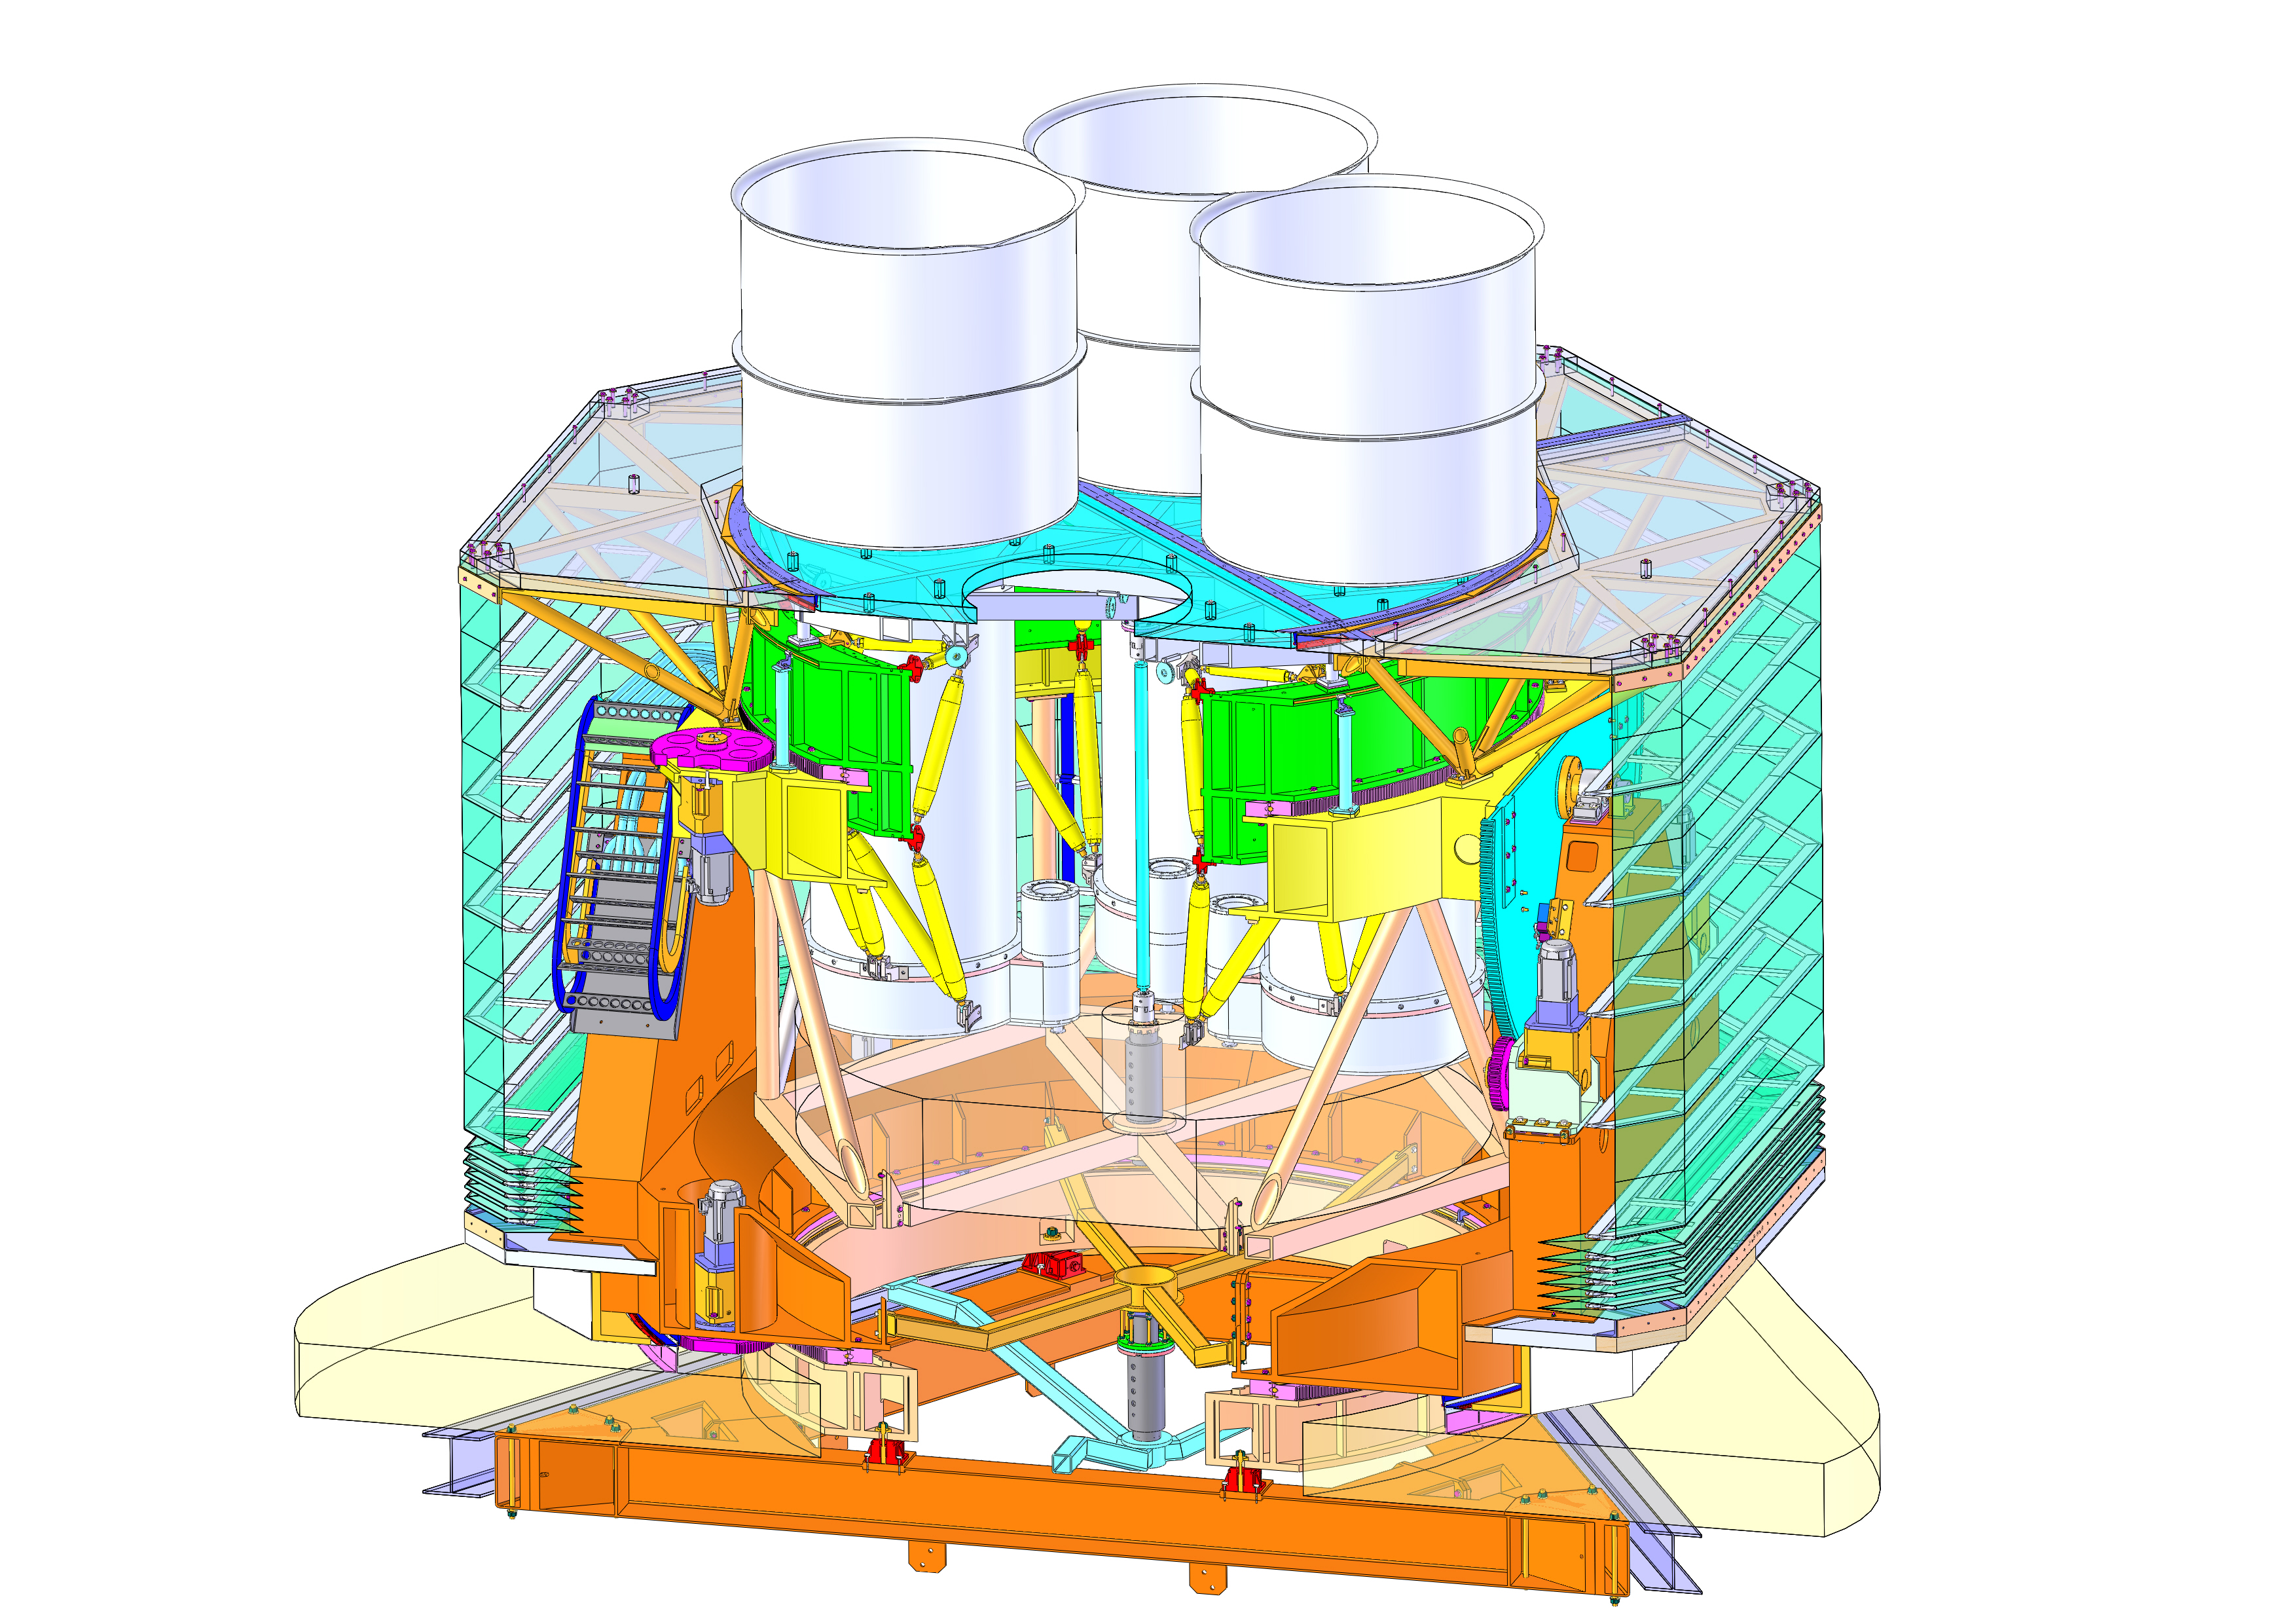
\includegraphics[scale=0.4]{BA_mount_isosection.JPG}
	\end{center}
	\caption{A CAD rendering of the new Bicep Array. The surrounding
	accordion-like environmental shield is shown in teal while the two rotary
	unions are depicted in gray and can be seen along the central axis of the
	mount.}
	\label{fig:bamount}
\end{figure}



% References
\bibliography{report} % bibliography data in report.bib
\bibliographystyle{spiebib} % makes bibtex use spiebib.bst

\end{document} 
